\let\negmedspace\undefined
\let\negthickspace\undefined
\documentclass[journal]{IEEEtran}
\usepackage[a5paper, margin=10mm, onecolumn]{geometry}
\usepackage{lmodern} 
\usepackage{tfrupee} 
\setlength{\headheight}{1cm}
\setlength{\headsep}{0mm}   

\usepackage{gvv-book}
\usepackage{gvv}
\usepackage{cite}
\usepackage{amsmath,amssymb,amsfonts,amsthm}
\usepackage{algorithmic}
\usepackage{graphicx}
\usepackage{textcomp}
\usepackage{xcolor}
\usepackage{txfonts}
\usepackage{listings}
\usepackage{enumitem}
\usepackage{mathtools}
\usepackage{gensymb}
\usepackage{comment}
\usepackage[breaklinks=true]{hyperref}
\usepackage{tkz-euclide} 
\usepackage{listings}                             
\def\inputGnumericTable{}                                 
\usepackage[latin1]{inputenc}                                
\usepackage{color}                                            
\usepackage{array}                                            
\usepackage{longtable}                                       
\usepackage{calc}                                             
\usepackage{multirow}                                         
\usepackage{hhline}                                           
\usepackage{ifthen}                                           
\usepackage{lscape}
\usepackage{xparse}

\bibliographystyle{IEEEtran}

\title{1.10.25}
\author{EE25BTECH11059 - Vaishnavi Ramkrishna Anantheertha}

\begin{document}
\maketitle

\renewcommand{\thefigure}{\theenumi}
\renewcommand{\thetable}{\theenumi}

\numberwithin{equation}{enumi}
\numberwithin{figure}{enumi} 

\textbf{Question}:
If a line makes angles $90^\circ$, $60^\circ$, and $30^\circ$ with the positive directions of the $X$, $Y$, and $Z$ axes respectively, find its direction cosines.
\\
\textbf{Solution: }\\
Definition of Direction Cosines: Direction cosines are the cosine values of the angles a vector makes with the $x$, $y$, and $z$ axes; they are the components of the unit vector along $x$,$y$,$z$ axes \\
\begin{table}[H]    
  \centering
  \begin{tabular}{|c|c|c|c|}
\hline
Angle (\(\alpha\)) & \(\cos(\alpha)\) & Value & Axis \\
\hline
\(90^\circ\) & \(\cos(90^\circ) = 0\) & \(l = 0\) & x-axis \\
\(60^\circ\) & \(\cos(60^\circ) = \frac{1}{2}\) & \(m = \frac{1}{2}\) & y-axis \\
\(30^\circ\) & \(\cos(30^\circ) = \frac{\sqrt{3}}{2}\) & \(n = \frac{\sqrt{3}}{2}\) & z-axis \\
\hline
\end{tabular}
  \caption{Variables Used}
  \label{tab:1.10.25}
\end{table}
Let the direction cosines be 
$l$,$m$,$n$\\
$l$,$m$,$n$, which are the cosines of the angles that the line makes with the $X$, $Y$, and $Z$ axes respectively.\\
\begin{align}
       l = \cos(90^\circ) = 0  \\
       m = \cos(60^\circ) = \frac{1}{2}  \\
       n = \cos(30^\circ) = \frac{\sqrt{3}}{2}   
\end{align}

A key property is that the sum of the squares of the direction cosines equals$1$:
\begin{center}
    $ l^2 + m^2 + n^2 = 1 $
\end{center}    

\begin{align}
\text{unit vector in direction of} \vec{x}= \myvec{
                                             0
                                              \\
                                               \frac{1}{2}
                                               \\
                                               \frac{\sqrt{3}}{2}
                                              }
\end{align}


Refer to Figure

\begin{figure}[H]
\begin{center}
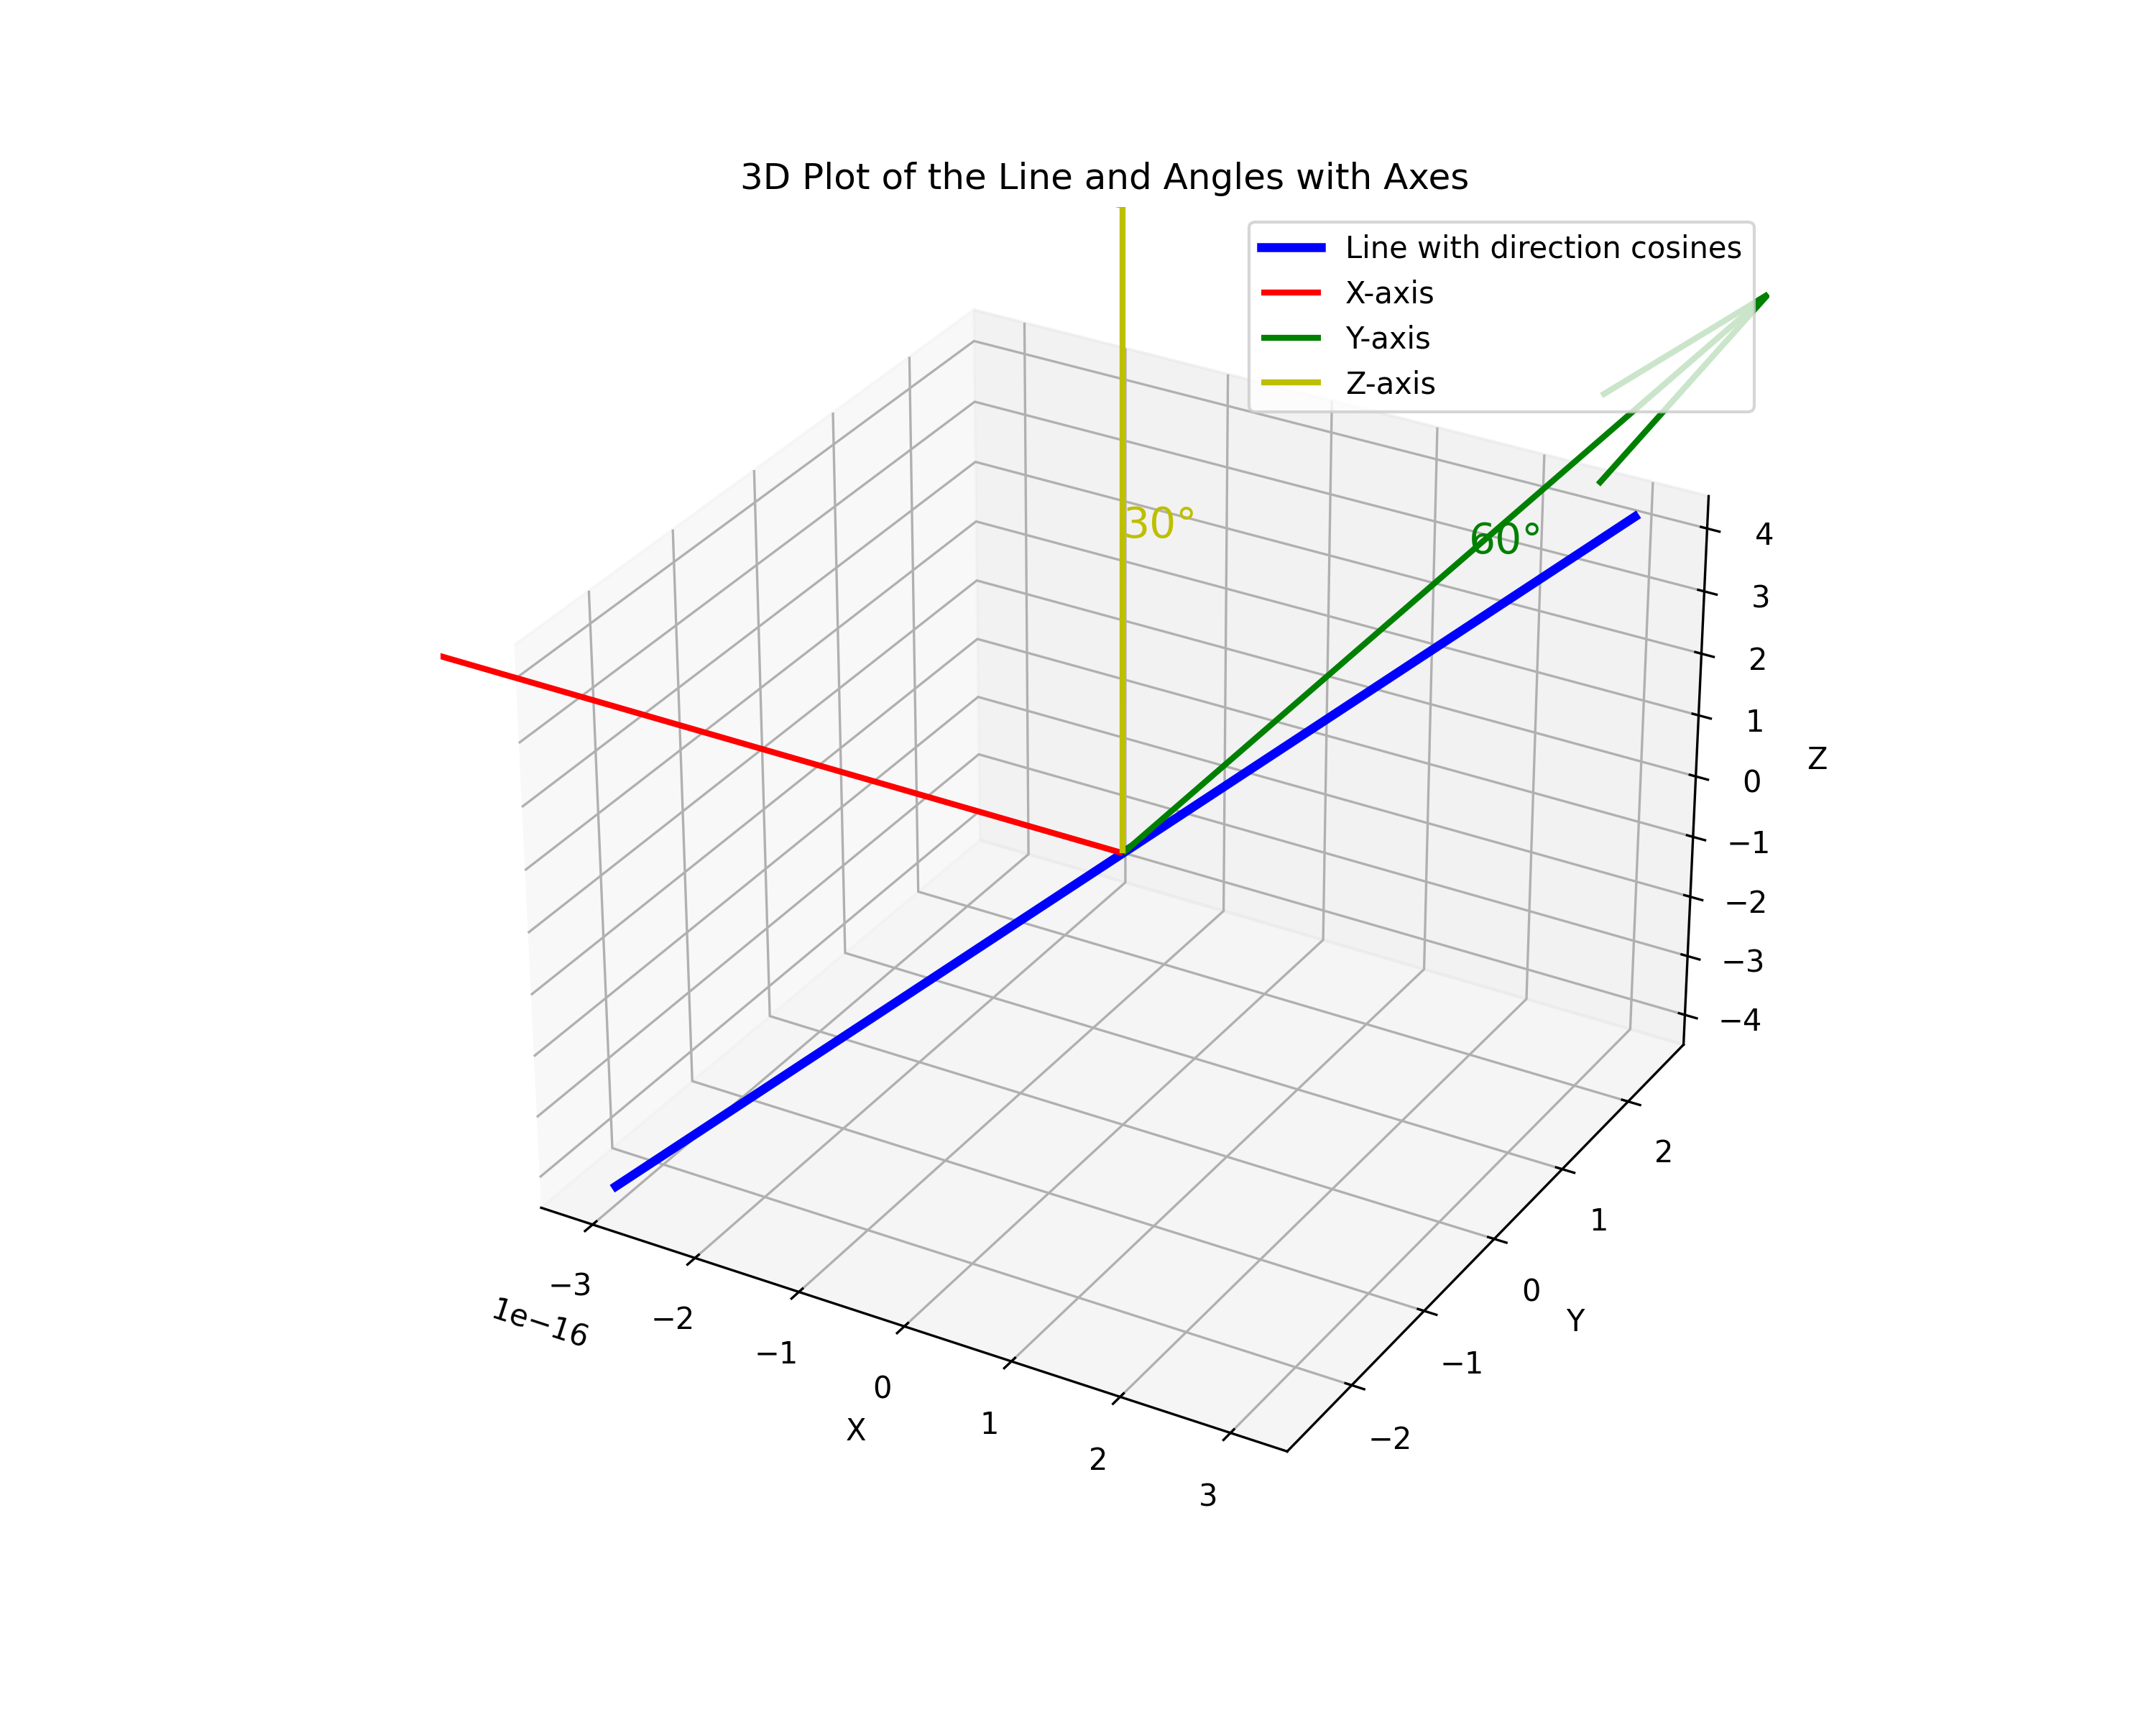
\includegraphics[width=0.6\columnwidth]{figs/graph2.png}
\end{center}
\caption{}
\label{fig:Fig}
\end{figure}
\end{document}  